\section{Wstęp}
%Część ta~zawiera wstępne informacje o~realizowanym projekcie. Zebrano w~nim wszystko to~co było dostępne zanim student przystąpił do~realizacji informatycznej części projektu. Opisano stanowisko laboratoryjne na~którym powstał projekt.

%\subsection{Geneza}
Tematem projektu, którego dotyczy ta praca jest: „System sterowania i wizualizacji pracy robota 3D". Pomysł na~projekt inżynierski pojawił się po~zrealizowaniu przez autora projektu semestralnego z~przedmiotu Sterowniki PLC. Zagadnienia związane z~tworzeniem oprogramowania dla sterowników przemysłowych są dla autora niezwykle interesujące, a zrealizowany projekt miał na~celu dalsze pogłębienie jego wiedzy z tego zakresu. Wyboru tego konkretnego tematu autor dokonał, ponieważ magazyny wysokiego składowania są~dosyć powszechną problematyką branży informatyki przemysłowej, a~praca nad tym tematem wydaje się być pomocna i~wartościowa w przyszłej pracy zawodowej lub na~dalszym etapie kształcenia.
%Po~podjęciu decyzji o~dziedzinie informatyki z~której projekt wydaje się interesujący przyszedł czas na~poszukiwania konkretnego tematu. Wybór padł na~ten konkretny temat ze~względu na~to, że~magazyny wysokiego składowania są~dość powszechną problematyką branży informatyki przemysłowej.

%\subsection{Temat}
%System sterowania i wizualizacji pracy robota 3D. \\
Głównymi celami pracy było napisanie oprogramowania dla sterownika przemysłowego Siemens S7-300 oraz stworzenie graficznej prezentacji pracy modelu Robota~3D takiego jak na~Rysunku~\ref{robot}.
Dodatkowym elementem pracy inżynierskiej zrealizowanej przez autora jest element pozainformatyczny, a mianowicie zbudowanie magazynu, z~którym robot będzie współpracował. Wyżej wspomniany magazyn po zakończeniu projektu posłuży jako pomoc dydaktyczna do~ćwiczeń laboratoryjnych.
\begin{figure}[!htb] \centering 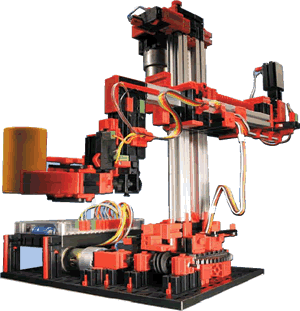
\includegraphics[width=0.4\textwidth]{obrazki/Fischertechnik3DRobot.png} \caption{Robot 3D firmy Fischertechnik} \label{robot} \end{figure}

\subsection{Stanowisko laboratoryjne}
\begin{figure}[!htb] 	\centering 	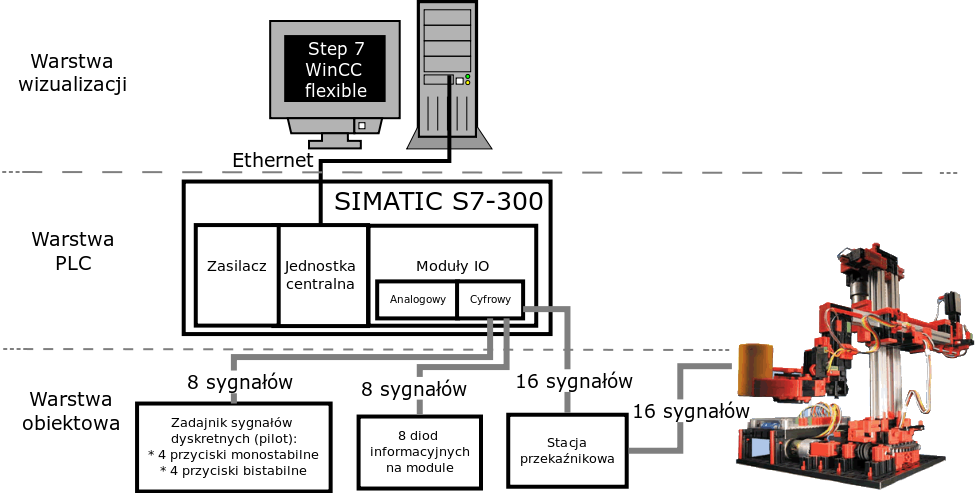
\includegraphics[width=0.99\textwidth]{obrazki/schemat.png} 	\caption{Schemat stanowiska} \label{schemat} \end{figure} 
Na potrzeby realizacji projektu wykorzystano istniejące stanowisko laboratoryjne, którego schemat przedstawia Rysunek~\ref{schemat}. Składa się ono~z:
\begin{itemize}
\item Sterownika PLC,
\item Komputera,
\item Modelu Robota 3D.
\end{itemize}
\indent
\indent Stanowisko to na potrzeby projektu rozbudowano o model magazynu wysokiego składowania. Poszczególne składowe stanowiska zostały bardziej szczegółowo opisane w~kolejnych podrozdziałach.
\subsubsection{Sterownik PLC}
Sterownik PLC wykorzystywany do realizacji projektu był wyposażony w następujące moduły:
\begin{enumerate}
\item SIMATIC S7-300, Jednostka centralna S7-300 CPU 315F-2 PN/DP,
\item SIMATIC S7-300, Zasilacz PS 307,
\item SIMATIC S7-300, Wejścia/Wyjścia cyfrowe SM 323,
\item SIMATIC S7-300, Wejścia/Wyjścia analogowe SM 334.
\end{enumerate}
\begin{figure}[!htb] 	\centering 	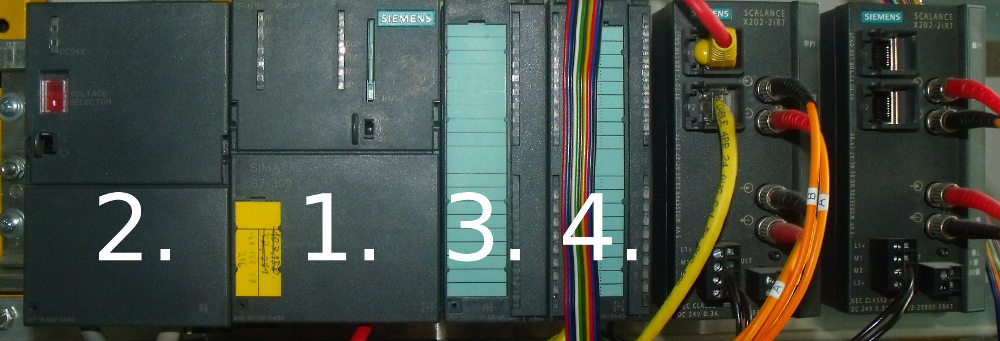
\includegraphics[width=0.75\textwidth]{obrazki/sterownik.png} 	\caption{Siemens SIMATIC S7-300} \end{figure}
\indent
\indent Sterownik podłączony jest do sieci lokalnej Ethernet w~laboratorium, więc komunikacja z~nim odbywa się tak samo jak z~każdym innym urządzeniem sieciowym. Podstawy programowania i korzystania ze sterowników autor poznał zapoznając się z odpowiednią literaturą \cite{plc1,plc2,plc4,plc5,plc6}.
Konfigurację sterownika wraz z modułami przedstawia Rysunek~\ref{conf}.
\begin{figure}[!htb] 	\centering 	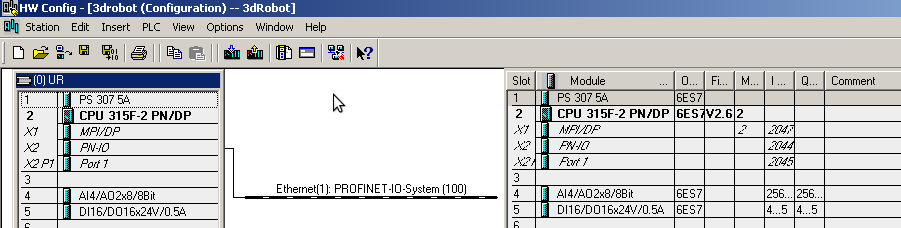
\includegraphics[width=0.75\textwidth]{obrazki/conf.png} \caption{Konfiguracja sterownika PLC} \label{conf} \end{figure}
\subsubsection{Komputer}
Projekt w całości był realizowany na laptopie autora, podłączanym do~sieci w~laboratorium. Na~komputerze uruchomiane były dwie maszyny wirtualne. Na~jednej zainstalowane było środowisko Step~7 do~programowania sterownika, a~na~drugiej WinCC flexible 2008 do~tworzenia i~uruchamiania wizualizacji. Wizualizacje tworzone w środowisku WinCC flexible są~dedykowane do~paneli operatorskich, jednak ta~stworzona przez autora na~potrzeby projektu była uruchamiana na komputerze za~pomocą runtime system.

\subsubsection{Model Robota 3D}
Wszelkie informacje dotyczące modelu robota zostały zebrane na podstawie obserwacji dokonanych przez autora oraz na podstawie udostępnionych przez uczelnię dokumentacji robota i instrukcji laboratoryjnej \cite{robot1,robot2}.

Model poprzez odpowiednie wysterowanie potrafi wykonać następujące ruchy: obracać się wokół własnej osi o 180 stopni, opuszczać i~podnosić, wysuwać i~wsuwać ramię oraz chwytać przedmioty. Każda z wymienionych funkcji jest realizowana przy użyciu odpowiedniego silnika. W dalszej części pracy silniki te będą nazywane odpowiednio: silnik Rotate, silnik Lift, silnik Arm oraz silnik Grab. Każdy element ruchomy robota jest wyposażony w~następujące czujniki:
\vspace*{-1mm}
\begin{enumerate}
\item „Wyłącznik krańcowy", sygnalizujący pozycję zerową (nazywany w~dalszej części pracy dla uproszczenia „krańcówką"). 
\vspace*{-1mm}
\item „Impulsator", czyli prosty enkoder informujący o pracy danego silnika i generujący 4 sygnały na każdy pełny obrót wału silnika.
\end{enumerate}
\vspace*{-1mm}
\indent
\indent Ponadto robot jest wyposażony w~cztery pary sygnałów 'Kierunek' oraz 'Praca silnika' po jednej dla każdego silnika. Sygnały wejściowe, pochodzące z~zadajnika sygnałów dyskretnych (nazywanego w~dalszej części pracy dla ułatwienia „pilotem") służą do sterowania modelem robota w trybie ręcznym. Model jest sterowany poprzez skrzynkę przekaźnikową (dostępną już na~stanowisku), która ma za~zadanie zmianę polaryzacji napięcia na silniku każdego elementu. Każdy silnik obsługiwany jest przez dwa przekaźniki.

Jak zostało pokazane na Rysunku~\ref{schemat}, linia sygnałów wychodząca z~modelu robota jest przekazywana do~skrzynki przekaźnikowej, w~której sygnały wejściowe (sygnały krańcówek) są przesyłane wprost do~stacji I/O (t.j. 8~sygnałów + 1~przewód wspólny, czyli masa dla sygnałów wejściowych). Sygnały wyjściowe (załączające silnik) w~skrzynce przekaźnikowej dołączone są do~przekaźników, które mają za~zadanie zmianę polaryzacji napięcia sterującego silnikami. Ze~skrzynki do~wyjść modułu~I/O dochodzą sygnały, które sterują zmianą polaryzacji na~wyjściach przekaźników oraz podaniem zasilania załączającego silnik (t.j. 8~sygnałów + 1~masa). Szczegóły dotyczące tych sygnałów zawierają Tablice~\ref{in}~oraz~\ref{out}.
%\vspace*{-2mm}
\begin{table}[!htb]
\begin{center}
\begin{comment}
\begin{tabular}{|c|c|c|l|}\hline
Nazwa  & Adres  & Typ  & Opis  \\   
zmiennej  & zmiennej & zmiennej  &   \\   
 & w sterowniku &  & \\\hline    
Rotate Manual Start  &   I       4.0 & Bool  &    Sterowanie ręczne Rotate - start.   \\\hline                                            
Arm Manual Start   &     I       4.1 &  Bool   &   Sterowanie ręczne Arm - start.      \\\hline                                            
Lift Manual Start   &    I       4.2 &  Bool   &   Sterowanie ręczne Lift - start.             \\\hline                                    
Grab Manual Start   &    I       4.3 &  Bool   &   Sterowanie ręczne Grab - start.             \\\hline                                    
Rotate Manual Dir   &    I       4.4 &  Bool   &   Sterowanie ręczne Rotate - kierunek.        \\\hline                                    
Arm Manual Dir      &    I       4.5 &  Bool   &   Sterowanie ręczne Arm - kierunek.           \\\hline                                    
Lift Manual Dir     &    I       4.6 &  Bool   &   Sterowanie ręczne Lift - kierunek.                                              \\\hline
Grab Manual Dir     &    I       4.7 &  Bool   &   Sterowanie ręczne Grab - kierunek.                                              \\\hline
Rotate Stop Sensor  &    I       5.0 &  Bool   &   Krańcówka wyłączająca dany silnik.                                              \\\hline
Rotate Counter      &    I       5.1 &  Bool   &   Krańcówka licznika impulsów \\ & & & dla obracania.                                      \\\hline
Arm Stop Engine Sensor & I       5.2 &  Bool  &    Krańcówka wyłączająca dany silnik.                                              \\\hline
Arm Engine Counter  &    I       5.3 &  Bool  &    Krańcówka licznika impulsów \\ & & & dla ramienia.                                       \\\hline
Lift Stop Sensor     &   I       5.4 &  Bool   &   Krańcówka wyłączająca dany silnik.                                              \\\hline
Lift Counter        &    I       5.5 &  Bool   &   Krańcówka licznika impulsów \\ & & & dla podnośnika.                                     \\\hline
Grab Sensor         &    I       5.6 &  Bool   &   Krańcówka wyłączająca dany silnik.                                              \\\hline
Grab Counter        &    I       5.7 &  Bool   &   Krańcówka licznika impulsów \\ & & & dla chwytaka.                                       \\\hline
\end{tabular}
\end{comment}
\begin{tabular}{|c|c| p{10cm} |}\hline
Adres zmiennej & Typ  & Opis \\
w sterowniku &  zmiennej &   \\\hline
I       4.0 & Bool  &    Sterowanie ręczne Rotate - start   \\\hline                                            
I       4.1 &  Bool   &   Sterowanie ręczne Arm - start      \\\hline                                            
I       4.2 &  Bool   &   Sterowanie ręczne Lift - start             \\\hline                                    
I       4.3 &  Bool   &   Sterowanie ręczne Grab - start             \\\hline                                    
I       4.4 &  Bool   &   Sterowanie ręczne Rotate - kierunek        \\\hline                                    
I       4.5 &  Bool   &   Sterowanie ręczne Arm - kierunek           \\\hline                                    
I       4.6 &  Bool   &   Sterowanie ręczne Lift - kierunek                                              \\\hline
I       4.7 &  Bool   &   Sterowanie ręczne Grab - kierunek                                              \\\hline
I       5.0 &  Bool   &   Krańcówka wyłączająca dany silnik                                              \\\hline
I       5.1 &  Bool   &   Krańcówka licznika impulsów dla obracania                                      \\\hline
I       5.2 &  Bool  &    Krańcówka wyłączająca dany silnik                                              \\\hline
I       5.3 &  Bool  &    Krańcówka licznika impulsów dla ramienia                                       \\\hline
I       5.4 &  Bool   &   Krańcówka wyłączająca dany silnik                                              \\\hline
I       5.5 &  Bool   &   Krańcówka licznika impulsów dla podnośnika                                     \\\hline
I       5.6 &  Bool   &   Krańcówka wyłączająca dany silnik                                              \\\hline
I       5.7 &  Bool   &   Krańcówka licznika impulsów dla chwytaka                                       \\\hline
\end{tabular}
\end{center}
\vspace*{-6mm}
  \caption{Zmienne wejściowe do modułów I/O}
	\label{in}
\end{table}
\begin{table}[!htb]
\begin{center}
\begin{comment}
\begin{tabular}{|c|c|c|l|}\hline
Nazwa  & Adres  & Typ  & Opis  \\   
zmiennej  & zmiennej & zmiennej  &   \\   
 & w sterowniku &  & \\\hline    
RotateMinValue    &      Q       4.0 &  Bool   &   Sygnalizacja osiągnięcia pozycji\\ & & &  minimalnej przez silnik Rotate.              \\\hline
RotateMaxValue     &     Q       4.1 &  Bool   &   Sygnalizacja osiągnięcia pozycji \\ & & & maksymalnej przez silnik Rotate.              \\\hline
ArmMinValue        &     Q       4.2  & Bool   &   Sygnalizacja osiągnięcia pozycji \\ & & &  minimalnej przez silnik Arm.                 \\\hline
ArmMaxValue        &     Q       4.3 &  Bool   &   Sygnalizacja osiągnięcia pozycji \\ & & &  maksymalnej przez silnik Arm.                 \\\hline
LiftMinValue       &     Q       4.4 &  Bool   &   Sygnalizacja osiągnięcia pozycji \\ & & &  minimalnej przez silnik Lift.                \\\hline
LiftMaxValue       &     Q       4.5  & Bool   &   Sygnalizacja osiągnięcia pozycji \\ & & &  maksymalnej przez silnik Lift.                \\\hline
GrabMinValue       &     Q       4.6  & Bool   &   Sygnalizacja osiągnięcia pozycji \\ & & &  minimalnej przez silnik Grab.                \\\hline
GrabMaxValue        &    Q       4.7 &  Bool   &   Sygnalizacja osiągnięcia pozycji \\ & & &  maksymalnej przez silnik Grab.                \\\hline
Rotate Engine On/Off &   Q       5.0 &  Bool   &   Włączenie/wyłączenie silnika \\ & & & obrotowego.                                       \\\hline
Rotate Left/Right   &    Q       5.1  & Bool   &   Kierunek obrotu \\ & & & (0-counterclock 1-clockwise).                                    \\\hline
Arm Engine On/Off    &   Q       5.2 &  Bool   &   Włączenie/wyłączenie silnika.                                                  \\\hline
Arm In/Out          &    Q       5.3  & Bool    &  Kierunek ramienia \\ & & & (0-In 1-Out).                                                 \\\hline
Lift Engine On/Off   &   Q       5.4  & Bool  &    Włączenie/wyłączenie silnika \\ & & & podnośnika (0-up 1-down).                         \\\hline
Lift Up/Down         &   Q       5.5  & Bool &     Kierunek podnoszenia.                                                           \\\hline
Grab On/Off         &    Q       5.6 &  Bool   &   Włączenie/wyłączenie silnika \\ & & & uchwytu.                                          \\\hline
Grab Close/Open    &     Q       5.7  & Bool  &    Kierunek chwytania \\ & & & (0-open 1-close).                                            \\\hline
\end{tabular}
\end{comment}
\begin{tabular}{|c|c| p{10cm} |}\hline
Adres zmiennej & Typ & Opis  \\
w sterowniku & zmiennej  &   \\\hline   
Q       4.0 &  Bool   &   Sygnalizacja pozycji minimalnej dla silnika \nobreak{Rotate}              \\\hline
Q       4.1 &  Bool   &   Sygnalizacja pozycji maksymalnej dla silnika \nobreak{Rotate}              \\\hline
Q       4.2  & Bool   &   Sygnalizacja pozycji minimalnej dla silnika Arm                 \\\hline
Q       4.3 &  Bool   &   Sygnalizacja pozycji maksymalnej dla silnika Arm                 \\\hline
Q       4.4 &  Bool   &   Sygnalizacja pozycji minimalnej dla silnika Lift                \\\hline
Q       4.5  & Bool   &   Sygnalizacja pozycji maksymalnej dla silnika Lift                \\\hline
Q       4.6  & Bool   &   Sygnalizacja pozycji minimalnej dla silnika Grab                \\\hline
Q       4.7 &  Bool   &   Sygnalizacja pozycji maksymalnej dla silnika Grab                \\\hline
Q       5.0 &  Bool   &   Włączenie/wyłączenie silnika obrotowego                                       \\\hline
Q       5.1  & Bool   &   Kierunek obrotu (0-counterclock 1-clockwise)                                    \\\hline
Q       5.2 &  Bool   &   Włączenie/wyłączenie silnika wysuwu                                                 \\\hline
Q       5.3  & Bool    &  Kierunek ramienia (0-In 1-Out)                                                 \\\hline
Q       5.4  & Bool  &    Włączenie/wyłączenie silnika podnośnika (0-up 1-down)                         \\\hline
Q       5.5  & Bool &     Kierunek podnoszenia                                                           \\\hline
Q       5.6 &  Bool   &   Włączenie/wyłączenie silnika uchwytu                                          \\\hline
Q       5.7  & Bool  &    Kierunek chwytania (0-open 1-close)                                           \\\hline
\end{tabular}
\end{center}
\vspace*{-6mm}
  \caption{Zmienne wyjściowe z modułów I/O}
	\label{out}
\end{table}

\subsubsection{Magazyn}
Jak już zostało wspomniane we~wstępie, projekt miał pozostawić po~sobie coś więcej niż tylko oprogramowanie i~wizualizację, więc powstał model magazynu, który posłuży studentom jako pomoc dydaktyczna na~laboratoriach z~programowania sterownika Siemens do~sterowania robotem Fischertechnik.

Magazyn zaprojektowano tak, aby optymalnie wykorzystać konstrukcję robota. Przegrody w modelu magazynu zostały rozmieszczone na~półokręgu ze~względu na~półkolisty tor poruszania się ramienia w~poziomie.
%\begin{figure}[!htb] 	\centering 	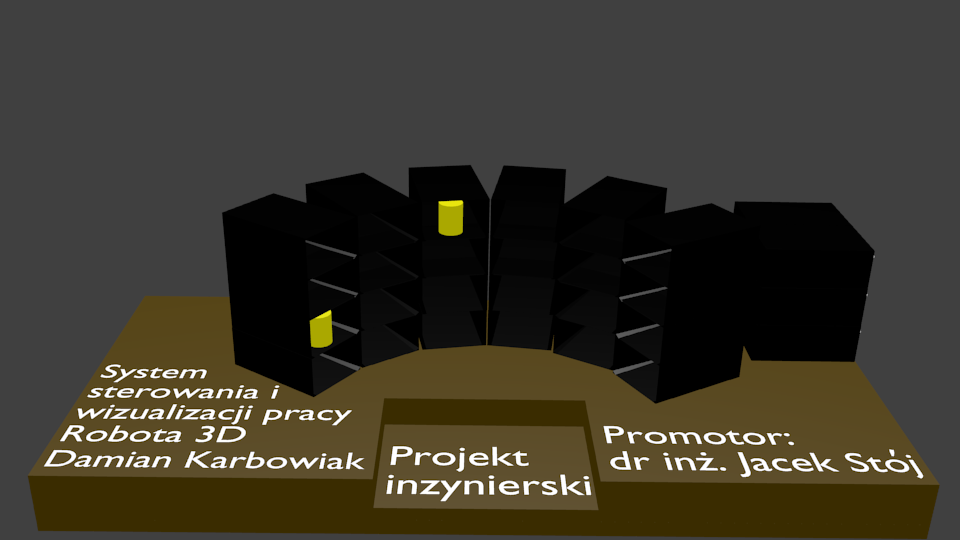
\includegraphics[width=0.95\textwidth]{obrazki/magazynb.png} 	\caption{Projekt magazynu wykonany w Blenderze}\end{figure}

Do budowy magazynu zastosowano płytę MDF o~grubości 18~mm oraz szufladki warsztatowe. Na~podstawie pomiarów wykonanych na~modelu oraz na~podstawie wcześniejszego projektu powstał model, który zobaczyć można na Rysunkach~\ref{mag}~oraz~\ref{mag2} lub w~sali~544 wydziału AEI na Politechnice Śląskiej.
\begin{figure}[!htb] 	\centering 	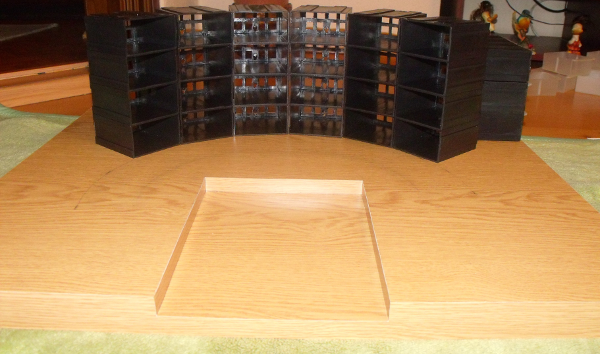
\includegraphics[width=0.55\textwidth]{obrazki/magazynr.png} \caption{Zbudowany magazyn} \label{mag} \end{figure}
\begin{figure}[!htb] 	\centering 	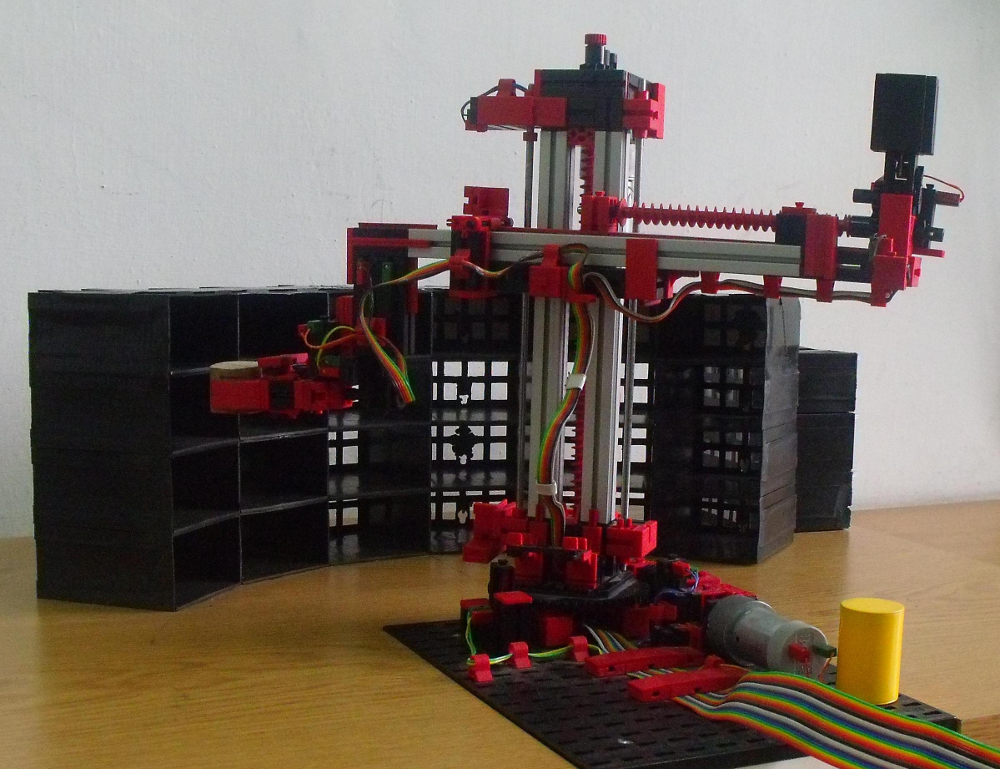
\includegraphics[width=0.7 \textwidth]{obrazki/magazynrobot.png} \caption{Zbudowany magazyn z zamontowanym robotem} \label{mag2} \end{figure}

\subsection{Analiza tematu}
Analiza tematu polegała przede wszystkim na zapoznaniu się z~narzędziami programistycznymi do~tworzenia oprogramowania sterownika oraz wizualizacji.
W~wyniku analizy autor poznał podstawy języków: LAD~\cite{step1,step2,step3}, STL~\cite{step1,step2,step3}, FBD~\cite{step1,step2,step3}, GRAPH~\cite{step3}, SCL~\cite{scl1,scl2,scl3} i AWL do~tworzenia programu sterownika oraz VBScript do~tworzenia skryptów w~wizualizacji. Poznanie tych podstaw pozwoliło dobrać język odpowiedni do~realizacji poszczególnych zadań.

\subsection{Założenia}
%Stworzone oprogramowanie dla Robota Fishertechnik ma działać na sterownikach firmy Siemens oraz ma zostać stworzone przy użyciu środowiska Step 7. Funkcjonalności robota, jakie mają wchodzić w~skład projektu, to:
Oprogramowanie dla Robota Fishertechnik powinno zostać stworzone przy użyciu środowiska Step 7 oraz działać na sterownikach firmy Siemens. Funkcjonalności robota wchodzące w~skład projektu, to:
\begin{itemize}
\item sterowanie ręczne z~pilota podłączonego bezpośrednio do~sterownika,
\item sterowanie ręczne z~wizualizacji,
\item sterowanie automatyczne, 
\item wizualizacja stanu magazynu,
\item umożliwienie korzystania z~magazynu zarówno poprzez sterowanie ręczne, jak i~przy użyciu zautomatyzowanych poleceń dostępnych z~poziomu wizualizacji.
\end{itemize}
\indent
\indent Powyżej zostały wymienione założenia podstawowe, jednak autor nie wyklucza zrealizowania dodatkowych zadań, które nie zostały zamieszczone w~pierwotnej koncepcji realizacji projektu.
%Zamieszczone tu założenia są podstawowe, ale niewykluczone jest zrealizowanie przez autora dodatkowych zadań nie zaplanowanych przed rozpoczęciem realizacji projektu.

\subsection{Plan pracy}
Realizacja projektu została podzielona na następujące etapy:
\begin{itemize}
\item Przygotowanie stanowiska, zebranie odpowiednich materiałów i~literatury,
\item Analiza wymagań funkcjonalnych aplikacji,
\item Projektowanie struktury oprogramowania i~interfejsów wymiany danych,
\item Implementacja,
\item Testowanie i~uruchamianie,
\item Przedstawienie projektu i~ewentualne korekty.
\end{itemize}
\indent
\indent Powyższy plan pracy stanowił dla autora wyznacznik kolejnych działań. Jednak powszechnie wiadomo, że w~praktyce poszczególne punkty są~wymienne i~wpływają na siebie wzajemnie.
